\documentclass[tikz,border=3mm]{standalone}
\usepackage[T1]{fontenc}
\usepackage{lmodern,amsmath,amssymb}
\usetikzlibrary{arrows.meta,calc,positioning,fit,backgrounds}
\definecolor{accent}{RGB}{36,91,158}
\definecolor{soft}{RGB}{225,237,248}
\definecolor{muted}{RGB}{122,134,145}
\definecolor{warm}{RGB}{250,242,220}
\tikzset{every node/.style={font=\sffamily\small},
vertex/.style={circle,draw=black!80,fill=white,minimum size=7.5mm,inner sep=1pt},
edge/.style={draw=accent!55,line width=.65pt},
highlight/.style={draw=accent,line width=1.7pt},
box/.style={draw=accent!70,rounded corners=2pt,fill=soft!45,align=center,inner sep=6pt},
heading/.style={font=\sffamily\bfseries\normalsize,align=center},
map/.style={-{Stealth[length=2mm]},line width=.8pt},
}
\hyphenpenalty=10000\exhyphenpenalty=10000
\begin{document}
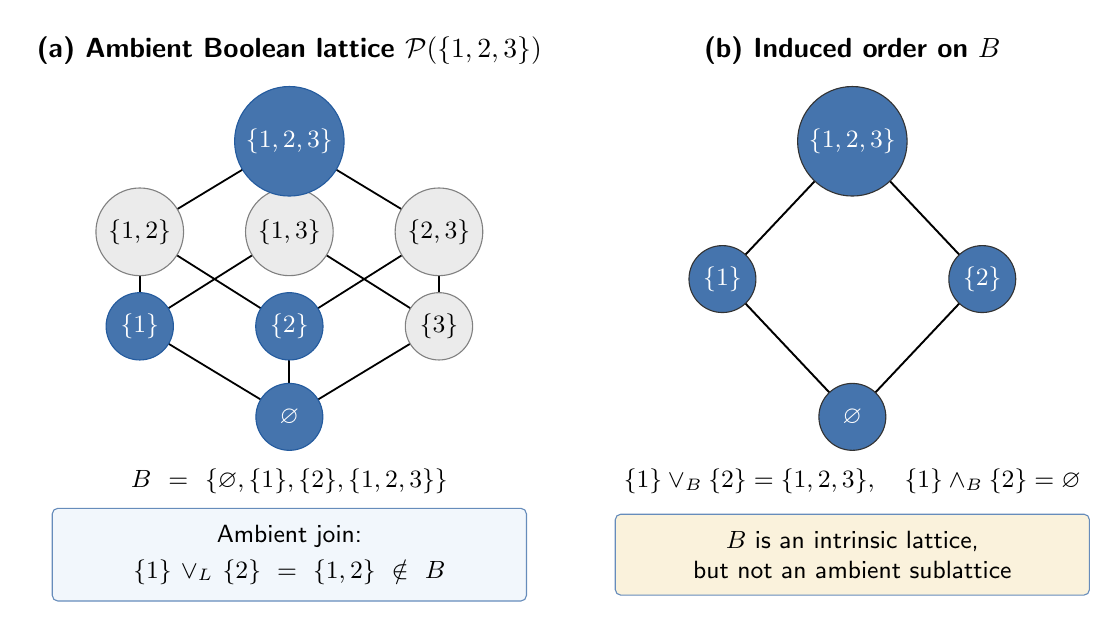
\begin{tikzpicture}[x=1cm,y=1cm]
\node[heading] at (0,5.9) {(a) Ambient Boolean lattice $\mathcal P(\{1,2,3\})$};
\coordinate (n0p) at (0,1.25);
\coordinate (n1p) at (-1.9,2.4);
\coordinate (n2p) at (0,2.4);
\coordinate (n3p) at (1.9,2.4);
\coordinate (n4p) at (-1.9,3.6);
\coordinate (n5p) at (0,3.6);
\coordinate (n6p) at (1.9,3.6);
\coordinate (n7p) at (0,4.75);
\draw[line width=.65pt] (n0p)--(n1p);
\draw[line width=.65pt] (n0p)--(n2p);
\draw[line width=.65pt] (n0p)--(n3p);
\draw[line width=.65pt] (n1p)--(n4p);
\draw[line width=.65pt] (n1p)--(n5p);
\draw[line width=.65pt] (n2p)--(n4p);
\draw[line width=.65pt] (n2p)--(n6p);
\draw[line width=.65pt] (n3p)--(n5p);
\draw[line width=.65pt] (n3p)--(n6p);
\draw[line width=.65pt] (n4p)--(n7p);
\draw[line width=.65pt] (n5p)--(n7p);
\draw[line width=.65pt] (n6p)--(n7p);
\node[vertex,fill=accent!85,text=white,draw=accent,minimum size=8.5mm,inner sep=2.8pt] at (n0p) {$\varnothing$};
\node[vertex,fill=accent!85,text=white,draw=accent,minimum size=8.5mm,inner sep=2.8pt] at (n1p) {$\{1\}$};
\node[vertex,fill=accent!85,text=white,draw=accent,minimum size=8.5mm,inner sep=2.8pt] at (n2p) {$\{2\}$};
\node[vertex,fill=black!8,draw=black!50,minimum size=8.5mm,inner sep=2.8pt] at (n3p) {$\{3\}$};
\node[vertex,fill=black!8,draw=black!50,minimum size=8.5mm,inner sep=2.8pt] at (n4p) {$\{1,2\}$};
\node[vertex,fill=black!8,draw=black!50,minimum size=8.5mm,inner sep=2.8pt] at (n5p) {$\{1,3\}$};
\node[vertex,fill=black!8,draw=black!50,minimum size=8.5mm,inner sep=2.8pt] at (n6p) {$\{2,3\}$};
\node[vertex,fill=accent!85,text=white,draw=accent,minimum size=8.5mm,inner sep=2.8pt] at (n7p) {$\{1,2,3\}$};
\node[align=center,text width=5.8cm] at (0,.43) {$B=\{\varnothing,\{1\},\{2\},\{1,2,3\}\}$};
\node[box,text width=5.6cm] at (0,-.50) {Ambient join:\\[2pt]$\{1\}\vee_L\{2\}=\{1,2\}\notin B$};
\node[heading] at (7.15,5.9) {(b) Induced order on $B$};
\coordinate (b0p) at (7.15,1.25);
\coordinate (b1p) at (5.5,3);
\coordinate (b2p) at (8.8,3);
\coordinate (b3p) at (7.15,4.75);
\draw[line width=.7pt] (b0p)--(b1p)--(b3p)--(b2p)--cycle;
\node[vertex,fill=accent!85,text=white,minimum size=8.5mm] at (b0p) {$\varnothing$};
\node[vertex,fill=accent!85,text=white,minimum size=8.5mm] at (b1p) {$\{1\}$};
\node[vertex,fill=accent!85,text=white,minimum size=8.5mm] at (b2p) {$\{2\}$};
\node[vertex,fill=accent!85,text=white,minimum size=8.5mm,inner sep=2.8pt] at (b3p) {$\{1,2,3\}$};
\node[align=center] at (7.15,.43) {$\{1\}\vee_B\{2\}=\{1,2,3\},\quad \{1\}\wedge_B\{2\}=\varnothing$};
\node[box,fill=warm,text width=5.6cm] at (7.15,-.50) {$B$ is an intrinsic lattice,\\but not an ambient sublattice};
\end{tikzpicture}
\end{document}
